\chapter{Radiation from Moving Charges}
\label{cha:radi-from-moving}
We will start to look at how radiation gets produced, scattered
and absorbed at a microscopic level to derive quantities like $j_\nu$,
$\alpha_\nu$ and $\sigma_\nu$.

\section{Retarded Potentials}
\label{sec:retarded-potentials}
\index{electrodynamics!retarded potentials}
We saw in the last section that in the Lorenz gauge the equations for
the vector and scalar potential are
\begin{equation}
\nabla^2 \phi - \frac{1}{c^2} \frac{\partial^2 \phi}{\partial t^2} =
-4\pi \rho,~~\hbox{\rm and}~~
  \nabla^2 {\bf A}
- \frac{1}{c^2} \frac{\partial^2 {\bf A}}{\partial t^2} =
-\frac{4\pi}{c} {\bf J}.
\label{eq:184}
\end{equation}
which have the following solution
\begin{eqnarray}
{\bf A}({\bf r},t) &=& \frac{1}{c} \int d^3 r' \frac{{\bf J}\left ({\bf
  r}',t-\frac{|{\bf r}-{\bf r}'|}{c} \right )}{|{\bf r} -
{\bf  r}'|} \\
\phi({\bf r},t) &=& \int d^3 r' \frac{\rho\left ({\bf
  r}',t-\frac{|{\bf r}-{\bf r}'|}{c} \right )}{|{\bf r} -
{\bf  r}'|} .
\label{eq:185}
\end{eqnarray}
An equivalent way of writing $\phi({\bf r},t)$ is
\begin{equation}
\phi({\bf r},t) = \int d^3 r' \int dt' \frac{\rho \left ({\bf
  r}',t'\right )}{|{\bf r} -
{\bf  r}'|} \delta ( t' - t + |{\bf r}-{\bf r}'|/c ) 
\label{eq:186}
\end{equation}
and similarly for ${\bf A}$

Let's think about a single charge with charge $q$ and position 
${\bf  r}_0(t)$.   It can be characterized by
\begin{equation}
\rho({\bf r},t) = q \delta({\bf r} -{\bf r}_0(t))~~\hbox{\rm
  and}~~{\bf j}(r, t) = q {\bf u} \delta({\bf r} - {\bf r}_0(t))
\label{eq:187}
\end{equation}
Let's substitute this expression for $\rho$,
\begin{eqnarray}
\phi({\bf r},t) &=& 
\int d^3 r' \int dt' \frac{q \delta({\bf r}'-{\bf r}_0(t'))}{|{\bf r} -
{\bf  r}'|} \delta ( t' - t + |{\bf r}-{\bf r}'|/c )  \\
 &=& 
q \int dt' \frac{1}{|{\bf r} -
{\bf  r}_0(t')|} \delta ( t' - t + |{\bf r}-{\bf r}_0(t')|/c )  
\label{eq:188}
\end{eqnarray}
It is easy to perform integrals over a $\delta$-function if the
integral is over the argument of the $\delta$-function, so we 
would like to perform the following change of variables
\begin{equation}
t'' = t' - t +  \frac{|{\bf r}-{\bf r}_0(t')|}{c}
\label{eq:189}
\end{equation}
yielding the Li\'enard-Wiechert potentials
\index{electrodynamics!Li\'enard-Wiechert potentials}
\begin{eqnarray}
\phi({\bf r},t) &=& 
q \int dt'' \frac{1}{|{\bf r} -
{\bf  r}_0(t')|} \delta ( t'' ) \frac{\partial t'}{\partial t''} \\
&=& \frac{q}{R(t_\rmscr{ret}) \kappa (t_\rmscr{ret})}\\
{\bf A} &=& \frac{q{\bf u}(t_\rmscr{ret})}{cR(t_\rmscr{ret}) \kappa (t_\rmscr{ret})}
\label{eq:190}
\end{eqnarray}
where
\begin{eqnarray}
R(t) &=& |{\bf r} - {\bf r}_0(t)| \\
t_\rmscr{ret} &=& t - \frac{R(t_\rmscr{ret})}{c} \\
\kappa(t) &=&  \frac{\partial t''}{\partial t'}.
\label{eq:191}
\end{eqnarray}
Let's look at the partial derivative now,
\begin{eqnarray}
\kappa(t) &=&  \frac{\partial t''}{\partial t'} = 1 + \frac{1}{c}
\frac{\partial R(t)}{\partial t}
\label{eq:192}
\end{eqnarray}
and looking at $R(t)$
\begin{equation}
R(t)^2 = {\bf R}(t) \cdot {\bf R}(t) 
\label{eq:193}
\end{equation}
so
\begin{equation}
2 R(t) {\dot R}(t) = -2 {\bf R}(t) \cdot {\bf u}(t) ~~\rmmat{NB:} ~~{\bf R} = {\bf r}-{\bf r}_0(t)
\label{eq:194}
\end{equation}
so
\begin{equation}
\kappa(t) = 1 - \frac{1}{c} \frac{{\bf R}(t) \cdot {\bf u}(t)}{R(t)} = 1 - \frac{1}{c} {\bf n}(t) \cdot {\bf u}(t).
\label{eq:195}
\end{equation}

\subsection{The Fields}
\label{sec:fields}
\index{electrodynamics!moving charges}
We can use the potentials to determine the electric and magnetic
fields produced by the moving particle.  Let us define
\begin{equation}
\betabold \equiv \frac{\bf u}{c},~\rmmat{so}~ \kappa = 1 - {\bf n} \cdot \betabold
\label{eq:196}
\end{equation}
which yield the fields (see \S~14.1 of Jackson)
\begin{eqnarray}
{\bf E}(r,t) &=& \kern-2mm q \left [ \frac{({\bf n} - \betabold)(1-\beta^2)}{\kappa^3 R^2} \right ]_\mathrm{ret}\!+\!\frac{q}{c} \left [ \frac{\bf n}{\kappa^3 R} \times \left [ 
({\bf n} - \betabold ) \times \dot{\betabold} \right ]\right ]_\mathrm{ret} \\
{\bf B}(r,t) &=& \kern-2mm\left [ {\bf n} \times {\bf E}(r,t) \right ]_\mathrm{ret}.
\label{eq:197}
\end{eqnarray}
It is important to remember that all of the properties of the particle
are evaluated at the retarded time.

A few things to notice are that if the particle is not accelerating
the electric field points to the current not the retarded position of
the particle.  This allows us to graphically depict the field for a
particle that is stopped suddenly.

The fields have two parts.  The first part is proportional to $1/R^2$
and it is simply a generalization of the field for a stationary
charge.  The second terms are proportional to $1/R$.  They are
\begin{eqnarray}
{\bf E}_\rmscr{rad}(r,t) &=& + \frac{q}{c} \left [ \frac{\bf n}{\kappa^3 R} \times \left [ 
({\bf n} - \betabold ) \times \dot{\betabold} \right ]\right ] \\
{\bf B}_\rmscr{rad}(r,t) &=& \left [ {\bf n} \times {\bf E}_\rmscr{rad}(r,t) \right ].
\label{eq:198}
\end{eqnarray}

\comment{
A fun thing to calculate is the Poynting vector of the fields for zero
acceleration
\begin{eqnarray}
{\bf S} &=&  \frac{c}{4\pi} {\bf E} \times {\bf B}\\
        &=&  \frac{c}{4\pi} \left ( {\bf E} \times ({\bf n} \times
        {\bf E} \right ) \\
	&=& \frac{c}{4\pi} \left [ {\bf n} \left ({\bf E} \cdot {\bf
        E}\right ) - {\bf E} \left ({\bf E}\cdot {\bf n} \right )
        \right ].
\label{eq:199}
\end{eqnarray}
Let's work through the first term,
\begin{equation}
{\bf n} \left ( {\bf E} \cdot {\bf E} \right ) = q^2 {\bf n} \frac{(1 - 2 {\bf n}\cdot
  \betabold + \beta^2)(1-\beta^2)^2}{\kappa^6 R^4}
\label{eq:200}
\end{equation}
Let's work on the second term now
\begin{eqnarray}
{\bf E} \left ( {\bf E} \cdot {\bf n} \right ) &=& q {\bf E} \left [ \frac{(1-\beta^2)}{\kappa^2 R^2}
  \right ] \\
&=&  q^2 \left [ \frac{({\bf n} - \betabold)(1-\beta^2)}{\kappa^3 R^2}
  \right ] 
 \left [ \frac{(1-\beta^2)}{\kappa^2 R^2}
  \right ] \\
&=& q^2  \frac{({\bf n} - \betabold)(1-\beta^2)^2}{\kappa^5 R^4}
\label{eq:201}
\end{eqnarray}
\begin{eqnarray}
{\bf S} &=&  \frac{c}{4\pi} 
\frac{q^2 (1-\beta^2)^2}{\kappa^6 R^4}
\left [ {\bf n} \left ( 1 - 2 {\bf n}\cdot \betabold + \beta^2 \right
  ) 
- \left ( {\bf n} - \betabold \right) \kappa \right ]\\
&=& \frac{c}{4\pi} 
\frac{q^2 (1-\beta^2)^2}{\kappa^6 R^4}
\left [ {\bf n} \left (  \betabold \cdot ( \betabold - {\bf n} )\right
  )
 + \betabold \kappa \right ]
\label{eq:202}
\end{eqnarray}
}

We can calculate the Poynting vector of the radiation fields
\begin{equation}
{\bf S} = {\bf n} \frac{q^2}{4\pi c \kappa^6 R^2} \left | {\bf n} \times
\left \{ \left ( {\bf n} - \betabold \right ) \times {\dot{\betabold}}
\right \} \right |^2
\label{eq:203}
\end{equation}

\subsection{Distribution in Frequency and Angle}
\label{sec:distr-freq-angle}

To examine the spectrum of the radiation let us define examine the
Fourier transform of the electric field.  We know (Eq.~\ref{eq:154})
\begin{equation}
\frac{dW}{dAd\omega} = c |\hat E(\omega)|^2
\label{eq:814}
\end{equation}
where
\begin{equation}
{\hat E} (\omega) = \frac{1}{2\pi} \int_{-\infty}^{\infty} E(t) e^{i\omega t} d t.
\label{eq:816}
\end{equation}
in our case we are interested in the energy emitted per solid angle so
\begin{equation}
\frac{dW}{d\Omega d\omega} = R^2 \frac{dW}{dA d\omega}= c |R \hat E(\omega)|^2
\end{equation}
and
\begin{equation}
R {\hat E} (\omega) = \frac{q}{2\pi c} \int_{-\infty}^{\infty}
\left [ \frac{\bf n}{\kappa^3} \times \left [ 
({\bf n} - \betabold ) \times \dot{\betabold} \right ]\right ]_\mathrm{ret}
e^{i\omega t} d t.
\label{eq:817}
\end{equation}
The intergrand is evaluated at the retarded time, $t'+R(t')/c=t$, so
we can change the variable of integration from $t$ to $t'$ to yield
\begin{equation}
R {\hat E} (\omega) = \frac{q}{2\pi c} \int_{-\infty}^{\infty}
\left [ \frac{\bf n}{\kappa^2} \times \left [ 
({\bf n} - \betabold ) \times \dot{\betabold} \right ]\right ]
e^{i\omega (t'+R(t')/c)} d t'.
\label{eq:818}
\end{equation}
If we assume that the observer is far away from where the acceleration
occurs, the unit vector ${\bf n}$ can be taken to be constant and
$R(t') \approx R_0 - {\bf n} \cdot {\bf r}(t')$, yielding
\begin{equation}
R {\hat E} (\omega) = \frac{q}{2\pi c} \int_{-\infty}^{\infty}
\left [ \frac{\bf n}{\kappa^2} \times \left [ 
({\bf n} - \betabold ) \times \dot{\betabold} \right ]\right ]
e^{i\omega (t'-{\bf n}\cdot {\bf r}(t')/c)} d t'.
\label{eq:819}
\end{equation} 
As we did earlier (\S~\ref{sec:spectrum}), the total energy radiated
per unit angle is
\begin{equation}
\frac{d W}{d\Omega d\omega} =
\frac{q^2}{4\pi^2 c} \left | \int_{-\infty}^{\infty}
\frac{{\bf n} \times \left [  ({\bf n} - \betabold ) \times
    \dot{\betabold} \right ]}{\left ( 1-\betabold\cdot {\bf n} \right )^2}
e^{i\omega (t'-{\bf n}\cdot {\bf r}(t')/c)} d t' \right |.
\label{eq:825}
\end{equation}
The expression can be simplied further by noticing that
\begin{equation}
\frac{{\bf n} \times \left [  ({\bf n} - \betabold ) \times
    \dot{\betabold} \right ]}{\left ( 1-\betabold\cdot {\bf n} \right
  )^2}
= \frac{d}{d t'} \left [ \frac{{\bf n} \times ({\bf n} \times
    \betabold ) }{1-\betabold\cdot {\bf n}} \right ].
\label{eq:820}
\end{equation}
and integrating Eq.~\ref{eq:819} by parts to yield
\begin{equation}
\frac{d W}{d\omega d\Omega} = \frac{q^2 \omega^2}{4\pi^2 c^3} 
\left | \int_{-\infty}^\infty {\bf n} \times ({\bf n} \times \betabold) e^{i
  \omega \left ( t'-{\bf n} \cdot {\bf r}_0 (t') / c \right )} dt'
\right |^2.
\label{eq:204}
\end{equation}

\subsection{Non-relativistic particles}
\label{sec:non-relat-part}
\index{electrodynamics!moving charges!non-relativistic}

Let's assume that $|\betabold| \ll 1$ and focus on a particular
frequency $\nu$ so that ${\dot u} \sim u \nu$.  We can compare the
``acceleration'' fields to the ``velocity'' field
\begin{eqnarray}
{\bf E}_\rmscr{acc} &=& \frac{q}{c^2 R} \left [ {\bf n} \times
    \left \{ {\bf n} \times \dot{\bf u} \right \} \right ] 
    \\
{\bf E}_\rmscr{vel} &=& \frac{q {\bf n}}{R^2}
\label{eq:205}
\end{eqnarray}
so
\begin{equation}
\frac{E_\rmscr{acc}}{E_\rmscr{vel}} \sim \frac{R \dot{u}}{c^2} \sim
\frac{R u \nu}{c^2} = \frac{u}{c} \frac{R}{\lambda}
\label{eq:206}
\end{equation}
so for points in the ``near zone'', $R\leq \lambda$, the velocity
field is stronger than the acceleration field by a factor $\geq c/u$; but
for points sufficiently far into the ``far zone'', $R\gg\ \lambda
(c/u)$, the acceleration field dominates.

Let's derive {\bf Larmor's formula} for the radiated energy.  Let use
the angle $\Theta$ to denote the angle between the vectors ${\bf n}$
and $\dot{{\bf u}}$, so we have
\begin{equation}
|{\bf E}_\rmscr{acc}| = |{\bf B}_\rmscr{acc}| = \frac{q \dot{u}}{Rc^2}
\sin \Theta
\label{eq:207}
\end{equation}
Using the formula for the Poynting vector we have
\begin{equation}
{\bf S} = {\bf n} \frac{c}{4\pi} E_\rmscr{acc}^2 = \frac{c}{4\pi}
\frac{q^2 \dot{u}^2}{R^2 c^3} \sin^2 \Theta
\label{eq:208}
\end{equation}
The power radiated per unit solid angle is simply $\left ( {\bf S}\cdot {\bf
  n}\right) R^2$ or
\begin{equation}
\frac{dW}{dt d\Omega} = \frac{q^2 \dot{u}^2}{4\pi c^3} \sin^2 \Theta
\label{eq:209}
\end{equation}
Let's integrate over all angles to get the power
\begin{eqnarray}
P &=& \frac{d W}{d t} = \frac{q^2 \dot{u}^2}{4\pi c^3} \int
\sin^2\Theta d\Omega = \frac{q^2 \dot{u}^2}{2 c^3}\int_{-1}^1 \left (1
- \mu^2 \right ) d \mu  \\
&=& \frac{2 q^2 \dot{u}^2}{3c^3}
\label{eq:210}
\end{eqnarray}

\subsection{How about relativistic particles?}
\label{sec:how-about-relat}
\index{electrodynamics!moving charges!relativistic}

Let's look at the Poynting vector again.
\begin{equation}
{\bf S} = {\bf n} \frac{q^2}{4\pi c \kappa^6 R^2} \left | {\bf n} \times
\left \{ \left ( {\bf n} - \betabold \right ) \times {\dot{\betabold}}
\right \} \right |^2
\label{eq:211}
\end{equation}
where ${\bf S}\cdot {\bf n}$ is the energy per unit area per unit time
detected at an observation poiint at time $t$ of radiation emitted by
the charge at time $t'=1-R(t')/c$.  Let's calculate the energy radiated away from $t'=T_1$ to $t'=T_2$ we would have
\begin{equation}
E = \int_{t=T_1+[R(T_1)/c]}^{t=T_2+[R(T_2)/c]}\left [{\bf S}\cdot {\bf n} \right ] d t
= \int_{T_1}^{T_2}\left [{\bf S}\cdot {\bf n} \right ] \frac{dt}{dt'} dt'
\label{eq:212}
\end{equation}
so we have
\begin{equation}
\frac{dP(t')}{d\Omega} = R^2 \left ({\bf S}\cdot {\bf n} \right )  \frac{dt}{dt'} = R^2  \left ({\bf S}\cdot {\bf n} \right ) \left ( 1 - \betabold \cdot n\right ) 
\label{eq:213}
\end{equation}
When we include the Poynting vector expression we have
\begin{equation}
\frac{dP(t')}{d\Omega} = \frac{q^2}{4\pi c} \frac{ \left | {\bf n} \times
\left \{ \left ( {\bf n} - \betabold \right ) \times {\dot{\betabold}}
\right \} \right |^2}{\left ( 1 - {\bf n} \cdot \betabold \right )^5}
\label{eq:214}
\end{equation}
Let's start by assuming the $\betabold$ is parallel to ${\dot{\betabold}}$, so  
$\betabold \times {\dot{\betabold}}=0$.  We get
\begin{equation}
\frac{dP(t')}{d\Omega} = \frac{q^2 {\dot u}^2}{4\pi c^3} 
\frac{ \sin^2 \Theta }{\left ( 1 - \beta \cos\Theta  \right )^5}
\label{eq:215}
\end{equation}
Let's integrate the power over all angles,
\begin{equation}
P = 2\pi \frac{q^2 {\dot u}^2}{4\pi c^2} \int_{-1}^1 
\frac{1-\mu^2}{\left ( 1 - \beta \mu \right )^5} d\mu = \frac{2}{3} \frac{q^2 {\dot u}^2}{c^2} \gamma^6
\label{eq:216}
\end{equation}
where
\begin{equation}
\gamma = \frac{1}{\sqrt{1-\beta^2}}=\frac{1}{\sqrt{(1+\beta)(1-\beta)}}
\label{eq:217}
\end{equation}
Let's take a second look at the angular distribution of power for small angles and 
$\beta \approx 1$.
\begin{eqnarray}
\frac{dP(t')}{d\Omega} &\approx&  \frac{q^2 {\dot u}^2}{4\pi c^3} 
\frac{ \theta^2 }{\left [ 1 - (1 - \gamma^{-2}/2 ) (1 - \theta^2/2 )
  \right ]^5} \\
&\approx &
 \frac{q^2 {\dot u}^2}{4\pi c^3} 
\frac{ \theta^2 }{\left [ \gamma^{-2}/2 + \theta^2/2   \right ]^5} \\
&\approx& \frac{8}{\pi}
 \frac{q^2 {\dot u}^2}{c^3} \gamma^8
\frac{ (\gamma \theta)^2 }{\left [ 1 + (\gamma \theta)^2   \right ]^5} 
\label{eq:218}
\end{eqnarray}
{
\begin{figure}
\centering
%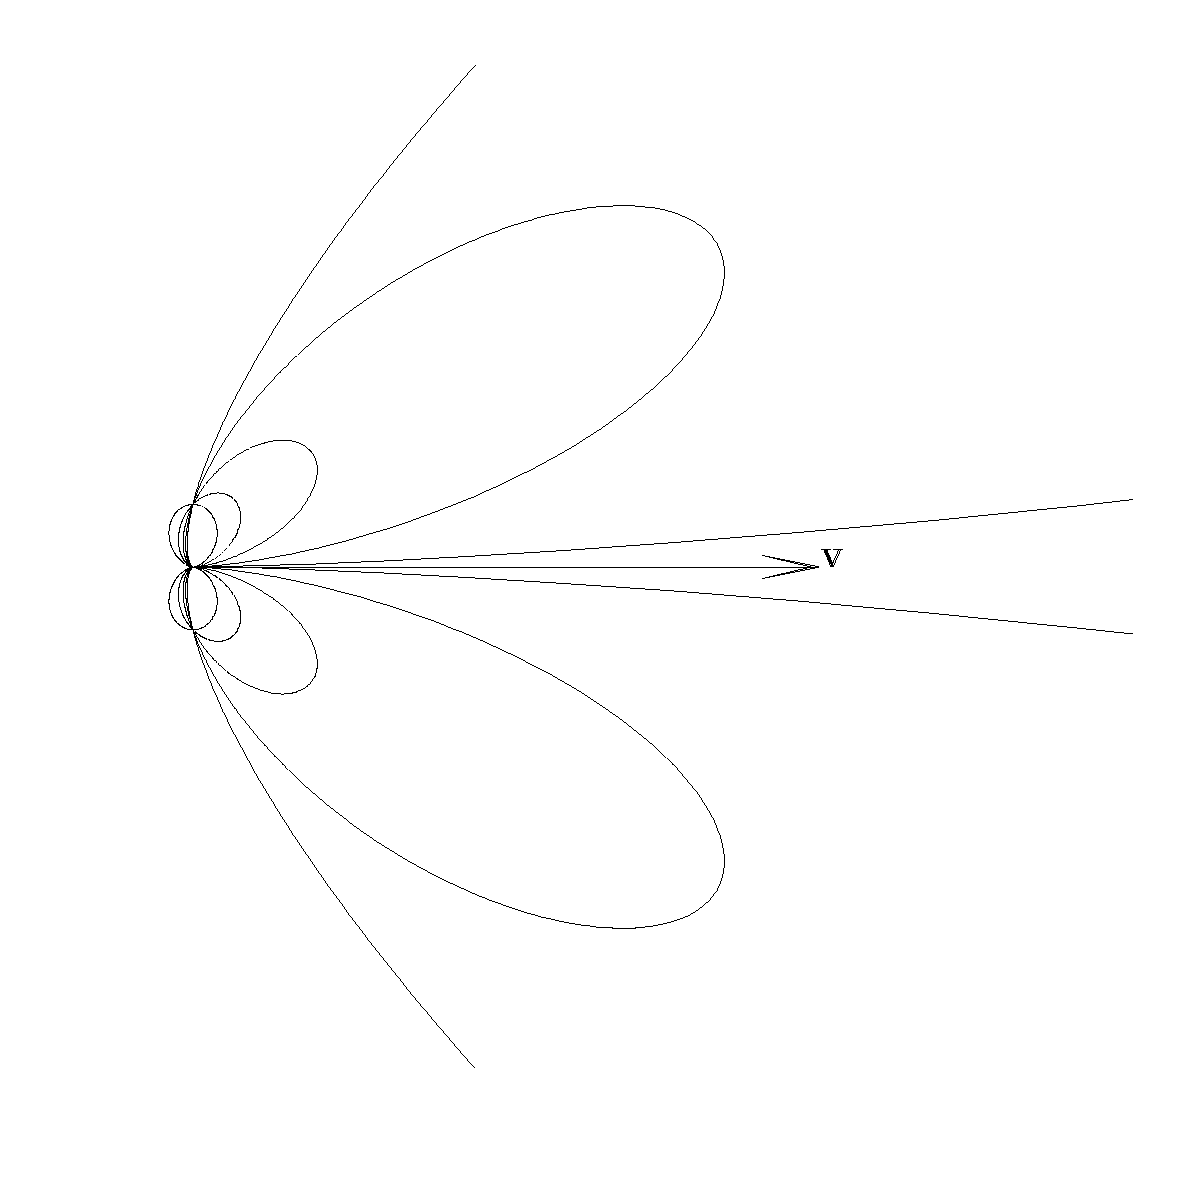
\includegraphics[width=0.45\textwidth]{sp}
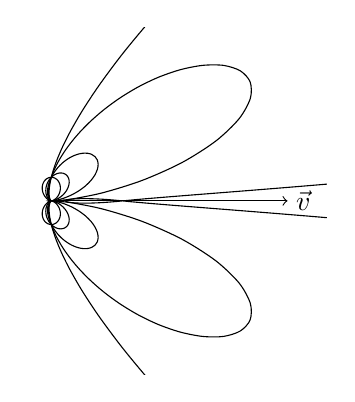
\begin{tikzpicture}
\clip (-0.3,-2.2) rectangle (3.5,2.2);
\foreach \b in {0, 0.2, 0.4, 0.6, 0.8} 
\draw plot [domain=0:360,smooth,samples=100] ( {-0.3*cos(\x)*sin(\x)^2/(1+\b*cos(\x))^5} ,
{0.3*sin(\x)^3/(1+\b*cos(\x))^5});
\draw [->] (0,0)--(3,0);
\draw (3.2,0) node {$\vec v$};
\end{tikzpicture}
% \includegraphics[width=0.45\textwidth]{rp2} 
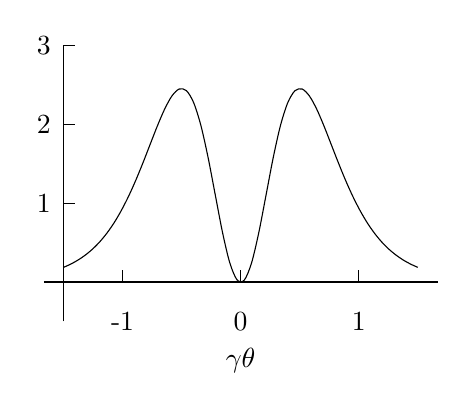
\begin{tikzpicture}
\draw plot [domain=-1.5:1.5,samples=50,smooth] ( {1.5*\x} , { \x*\x /
  (1+\x*\x)^5 *30 });
\draw  (-2.5,0)--(2.5,0) ;
\draw  (-2.25,-0.5)--(-2.25,3) ;
\draw (0,-1) node {$\gamma\theta$} ;
\foreach \x in { -1, 0, 1 }
  \draw (1.5*\x,-0.5) node {\x} (1.5*\x,0)--(1.5*\x,0.15);
\foreach \y in { 1, 2, 3 }  
  \draw (-2.5,\y) node {\y} (-2.25,\y) -- (-2.1,\y) ;
\end{tikzpicture}
\caption{Radiated power as a function of angle and $\gamma \theta$ for
  longitudinal motion. The left-hand panel shows from inside out
  $\beta=0,0.2,0.4,0.6,0.8$.}
\end{figure}
}

Let's repeat the calculation for circular motion, in which $\betabold
\perp {\dot{\betabold}}$.  To be definitive we have to specify two
angles for our observer ${\bf n}$.  Let's take the velocity to be
along the $z$-axis and the accelation along the $z$ axis, so $\Theta$
is the angle between ${\bf n}$ and the velocity and $\phi$ is the
angle between the projection of the vector ${\bf n}$ into the $x-y$-plane 
and the acceleration ({\em i.e.} these are just ordinary spherical coordinates). We obtain in general,
\begin{equation}
\frac{dP(t')}{d\Omega} = \frac{q^2 {\dot u}^2}{4\pi c^3} 
\frac{ 1 }{\left ( 1 - \beta \cos\Theta  \right )^3}
\left [ 1 - 
\frac{ \sin^2 \Theta \cos^2\phi }{\gamma^2 \left ( 1 - \beta \cos\Theta  \right )^2} \right ]
\label{eq:219}
\end{equation}
If we integrate this over all angles we get
\begin{equation}
P(t') = \frac{2}{3} \frac{q^2 {\dot u}^2}{c^3} \gamma^4
\label{eq:220}
\end{equation}
At first glance, the power from longitudinal motion seems much larger that the circular 
motion, but it is important to compare the power emitted for the same applied force ($d{\bf p}/dt$).

For circular motions the applied force is $\gamma m {\dot u}$, yielding
\begin{equation}
P_\rmscr{circ}(t') = \frac{2}{3} \frac{q^2}{m^2 c^3} \gamma^2 \left ( \frac{d {\bf p}}{d t}\right )^2
\label{eq:221}
\end{equation}
For longitudinal acceleration, the applied force is given by $m \gamma^3 {\dot u}$
\begin{equation}
P_\rmscr{long}(t') = \frac{2}{3} \frac{q^2}{m^2 c^3} \left ( \frac{d {\bf p}}{d t}\right )^2
\label{eq:222}
\end{equation}
For a given applied force, the radiation due to the component
perpendicular to the motion is much larger than the parallel
component.  If the particles are ultrarelativistic it is appropriate
to neglect the parallel contribution completely.

\subsection{Radiation from Systems of Particles}
\label{sec:radi-from-syst}

Let's focus back on the radiation from a non-relativistic particle,
specifically a bunch of such particles.  The electric field is linear
so the total electric field of the ensemble is the sum of the
particle's individual contributions,
\begin{equation}
{\bf E}_\rmscr{tot} = \sum_i
 \frac{q_i}{c^2 R_i} \left [ {\bf n}_i \times
    \left \{ {\bf n}_i \times \dot{\bf u}_i \right \} \right ] 
\label{eq:223}
\end{equation}
This sum could get really cumbersome, especially if you have $\sim
10^{40}$ particles.  You have to calculate the retarded position and
keep track of the velocity of each one.   There is an easier way.

Let's assume that the particles are confined to a region of size $l$
and we are really far from that region, $R_i \gg\ l$ so $R_i \approx
R$ where $R$ is the distance to the centre of the region and ${\bf n}_i
\approx {\bf n}$, a vector pointing to the centre of the region.

For the above expression for the electric field to be valid, $R/c$
must be greater than any timescale ($\tau$ for the particles to change
position ({\em i.e.} we are in the ``far'' zone).  Let's also assume that
$c\tau \gg\ l$ which means that we can neglect the difference in
retarded time between particles at one end of the region and the
other.  Let's make these changes
\begin{equation}
{\bf E}_\rmscr{tot} = \frac{1}{c^2 R} 
 \left [ {\bf n} \times
    \left \{ {\bf n} \times  \sum_i q_i \dot{\bf u}_i \right \} \right ] 
\label{eq:224}
\end{equation}
Let's define the dipole moment of the ensemble
\begin{equation}
{\bf d} = \sum_i q_i {\bf r}_{0,i}
\label{eq:225}
\end{equation}
which yields
\begin{equation}
{\bf E}_\rmscr{tot} = \frac{1}{c^2 R} 
 \left [ {\bf n} \times
    \left \{ {\bf n} \times  \ddot {\bf d} \right \} \right ] 
\label{eq:226}
\end{equation}
We also get
\begin{equation}
\frac{d P}{d \Omega} = \frac{\ddot{\bf d}^2}{4\pi c^3} \sin^2 \Theta
~~\rmmat{and}~~ P=\frac{2 \ddot{\bf d}^2}{3c^3}
\label{eq:227}
\end{equation}
Let's examine the spectrum of dipole radiation.  To make things
easier, let us assume that the dipole lies in a single direction and
varies in magnitude (imagine a negative charge moving up and down a
wire).  In this case the electric field is parallel to ${\bf d}$ and
we have
\begin{equation}
E(t) = \ddot{d} (t) \frac{\sin \Theta}{c^2 R}
\label{eq:228}
\end{equation}
Let's define 
\begin{equation}
d(t) = \int_{-\infty}^\infty e^{-i\omega t} {\hat d}(\omega) d \omega
\label{eq:229}
\end{equation}
so we have
\begin{equation}
\ddot{d}(t) = -\int_{-\infty}^\infty \omega^2 e^{-i\omega t} {\hat d}(\omega) d \omega
\label{eq:230}
\end{equation}
so
\begin{equation}
{\hat E}(\omega) = - \frac{1}{c^2 R_0} \omega^2 {\hat d}(\omega) \sin \Theta
\label{eq:231}
\end{equation}
and the power per unit solid angle and frequency is
\begin{equation}
\frac{dW}{d \omega d\Omega} = \frac{1}{c^3} \omega^4 |{\hat
  d}(\omega)|^2 \sin^2 \Theta ~\rmmat{and}~ \frac{dW}{d\omega} =
\frac{8\pi \omega^2}{3c^3} |{\hat d}(\omega)|^2
\label{eq:232}
\end{equation}

\subsection{A Physical Aside: Multipole Radiation}
\label{sec:phys-asid-mult}
\index{electrodynamics!multipole radiation}

It is possible to calculate the radiation field to higher order in
$L/(c\tau)$.  This is necessary if the dipole moment vanishes, for
example.   We can expand the exponential to yield
\begin{equation}
A_\omega ({\bf r}) = \frac{e^{ikr}}{cr} \sum_{n=0}^\infty \frac{1}{n!}
\int {\bf j}_\omega ({\bf r}') \left ( -ik{\bf n}\cdot {\bf r}' \right
)^n d^3 r'
\label{eq:233}
\end{equation}
where $k\equiv\omega/c$  $n=0$ gives the dipole radiation, $n=1$ gives
the quadrupole radiation and so on.

\section{Cherenkov Radiation}
\label{sec:cherenkov-radiation}
\index{electrodynamics!Cherenkov radiation}
\index{Cherenkov radiation}
\index{Cerenkov radiation}
\index{electrodynamics!moving charges!Cherenkov radiation}

\newcommand{\waves}[1]{
  \fill (0,0) circle (0.02);
  \draw [->,thick] (-1.6*#1,0)--(0,0) ;
  \draw [dashed] (-1.6*#1,0)--(-1.6*#1,-2.4) 
                 (0,0) -- (0,-2)
                 (-1.6*#1+1.6,0) -- (-1.6*#1+1.6,-2.4);
  \draw [<-] (-1.6*#1,-2.3) -- (-1.6*#1+0.6,-2.3) ;
  \draw [->] (-1.6*#1+1.0,-2.3) -- (-1.6*#1+1.6,-2.3) ;
  \draw (-1.6*#1+0.8,-2.3) node {$ct$};
  \draw [<-] (-1.6*#1,-1.9) -- (-0.8*#1-0.2,-1.9) ;
  \draw [->] (-0.8*#1+0.2,-1.9) -- (0,-1.9) ;
  \draw (-0.8*#1,-1.9) node {$vt$};
   \foreach \t in {0.2,0.4,...,1.6} \draw (-\t*#1,0) circle (\t);
}
\begin{figure}
\begin{center}
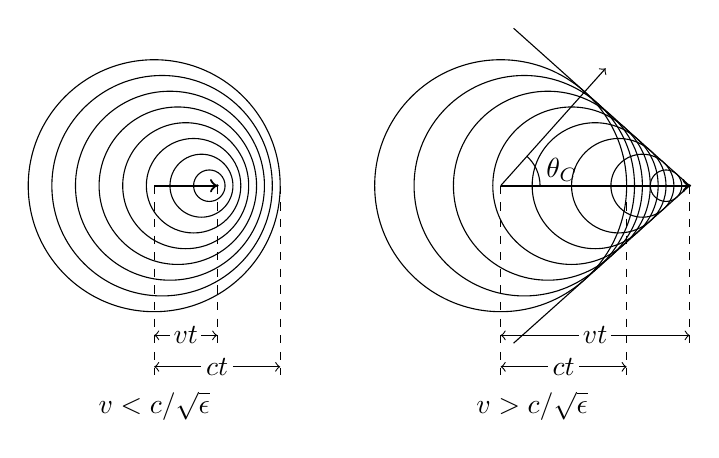
\begin{tikzpicture}
\waves{0.5}
\draw (-0.8,-2.8) node {$v<c/\sqrt{\epsilon}$};
\begin{scope}[shift={(6,0)}]
\waves{1.5}
\draw (-1.118033989*2,2) -- (0,0) -- (-1.118033989*2,-2);
\draw (-2,-2.8) node {$v>c/\sqrt{\epsilon}$};
\draw [->] (-2.4,0) -- ++(48.191106385:2);
\draw  (-1.9,0) arc (0:48.191106385:0.5);
\draw  (-2.4,0) ++(24.095553193:0.5) node [right] {$\theta_C$};
\end{scope}
\end{tikzpicture}
\end{center}
\caption{The propagation of electromagnetic waves from a source
  travelling slower and faster than the speed of light in the medium
  ($c/\sqrt{\epsilon}$ in \S~\ref{sec:cherenkov-radiation}).}
\label{fig:cherenkov}
\end{figure}

When a charge travels through a medium faster than the speed of light
in the medium (taken to be $c/\sqrt{\epsilon}$ in this section),
additional complications arise.  Fig.~\ref{fig:cherenkov} illustrates
how for $v<c/\sqrt{\epsilon}$ each point yields a unique retarded time
denoted by the circles.  On the other hand if $v>c/\sqrt{\epsilon}$
the space is divided into two regions.  In one outside the ``Cherenkov
cone'' one cannot assign a retarded time to a particular point and
within one must assign two different times to each point.  On the cone
one has a range of proper times.  We can translate our earlier
results, for example Eq.~\ref{eq:204}, by making the following
substitutions
\begin{equation}
c \rightarrow \frac{c}{\sqrt{\epsilon}}~\hbox{\rm and}~q \rightarrow \frac{q}{\sqrt{\epsilon}}
\end{equation}
yielding
\begin{equation}
\frac{d W}{d\omega d\Omega} = \frac{q^2 \omega^2 \epsilon^{1/2}}{4\pi^2 c^3} 
\left | \int_{-\infty}^\infty {\bf n} \times ({\bf n} \times \betabold) e^{i
  \omega \left ( t'- {\bf n} \cdot {\bf r}_0 (t') \epsilon^{1/2} / c \right )} dt'
\right |^2.
\label{eq:826}
\end{equation}
Here we have uniform motion in a straight line ${\bf r}(t')={\bf v}
t'$ so
\begin{equation}
\frac{d W}{d\omega d\Omega} = \frac{q^2 \epsilon^{1/2}}{c^3} 
|{\bf n} \times {\bf v}|^2 
\left | \frac{\omega}{2\pi} \int_{-\infty}^\infty e^{i
  \omega t' \left ( 1 - {\bf n} \cdot {\bf v} \epsilon^{1/2} / c \right )} dt'
\right |^2.
\label{eq:827}
\end{equation}
The integral is a Dirac delta function, so we have
\begin{equation}
\frac{d W}{d\omega d\Omega} = \frac{q^2 \epsilon^{1/2} \beta^2 \sin^2
  \theta}{c} 
\left | \delta ( 1 - \epsilon^{1/2} \beta \cos \theta)\right |^2
\label{eq:815}
\end{equation}
where $\theta$ is measured relative to the velocity of the particle.
The radiation is only emitted at the angle
\begin{equation}
\cos \theta_C = \frac{1}{\beta \epsilon^{1/2}}.
\end{equation}
In general the dielectric constant is a function of frequency and the
frequency dependence does not change the result of Eq.~\ref{eq:815},
so we also find that the radiation is only emitted 
at frequencies where $\beta\epsilon^{1/2}(\omega) > 1$, or to put it another
way at frequencies where the charge exceeds the propagation speed of
the radiation.

The total energy radiated according to Eq.~\ref{eq:815} diverges;
this simply results from our assumption that the charge travels
through the dielectric material forever and this assumption is easy to
relax by replacing the infinite integral with one over a time $2T$
during which the particle travels through the dielectric
\begin{equation}
\frac{\omega}{2\pi} \int_{-T}^T e^{i  \omega t' \left ( 1 - {\bf n}
    \cdot {\bf v} \epsilon^{1/2} / c \right )} dt' =
\frac{\omega T}{\pi} \frac{\sin \left [ \omega T \left ( 1 -
      \epsilon^{1/2} \beta \cos \theta \right ) \right ]}{\left [ \omega T \left ( 1 -
      \epsilon^{1/2} \beta \cos \theta \right ) \right ]}.
\end{equation}
Again the radiation is sharply peaked at the Cherenkov angle as long
as $\omega T \gg 1$ and we can integrate this result over all angles
to yield the total energy per frequency emitted as the charge travels
through the dielectric 
\begin{equation}
\frac{d W}{d\omega} = \frac{q^2 \omega}{c^2} \sin^2 \theta_c \left (2
  c \beta T \right ) = \frac{q^2 \omega}{c^2} \left [ 1 -
  \frac{1}{\beta^2 \epsilon(\omega)} \right ] \left ( 2 c \beta T
\right )
\end{equation}
where $2 c \beta T$ is the thickness of the dielectric region.

\section{Thomson Scattering}
\label{sec:thomson-scattering}
\index{electrodynamics!Thomson scattering}
\index{radiative transfer!Thomson scattering}
Let's imagine that an electromagnetic wave hits a charge particle causing it to move 
according to the Lorentz force equation,
\begin{equation}
{\bf F} = q \left ( {\bf E}_\rmscr{wave} 
+ \frac{\bf u}{c} \times {\bf B}_\rmscr{wave}  \right ).
\label{eq:234}
\end{equation}
To simplify matters let's assume that $u \ll\ c$ so we can neglect the
magnetic term because $E_\rmscr{wave}=B_\rmscr{wave}$ so we have.
\begin{equation}
\dot{\bf u} = \frac{q}{m} {\bf E}_\rmscr{wave} 
\label{eq:235}
\end{equation}
Because the wave is accelerated, it radiates electromagnetic radiation
\begin{equation}
{\bf E}_\rmscr{acc} = \frac{q^2}{c^2 m R} \left [ {\bf n} \times
    \left \{ {\bf n} \times {\bf E}_\rmscr{wave} \right \} \right ] 
\label{eq:236}
\end{equation}
The radiated wave has the same frequency content as the incident
wave.  The electric field of the radiated wave is in the plane
containing ${\bf E}_\rmscr{wave}$ and ${\bf n}$.
{
\begin{figure}
\centering
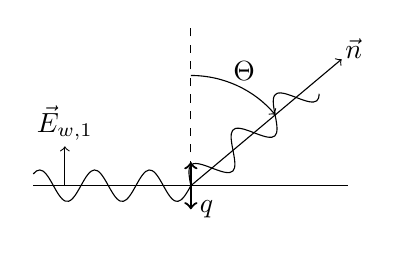
\begin{tikzpicture}
\draw (-2,0) -- (2,0) ;
\draw [dashed] (0,0) -- (0,2);
\draw [<->,thick] (0,-0.3) -- (0,0.3) ;
\draw  (0.2,-0.3) node {$q$};
\draw [->] (0,0) -- (40:2.5) ;
\draw (40:2.7) node {$\vec n$} ;
\draw [->] (90:1.4) arc (90:40:1.4) ;
\draw (65:1.6) node {$\Theta$} ;
\draw [->] (-1.6,0) -- (-1.6,0.5) ;
\draw (-1.6,0.8) node {$\vec E_{w,1}$} ;
\draw plot [domain=-2:0,smooth,samples=50] (\x, {0.2*sin(9*\x r)});
\draw plot [domain=0:2,smooth,samples=50] ({\x*0.7666-0.2*sin(9*\x r)*0.642}, {\x*0.642+0.7666*0.2*sin(9*\x r)});
\end{tikzpicture}
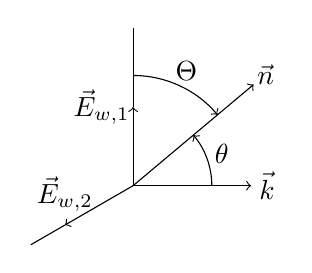
\begin{tikzpicture}
\draw [->] (0,0) -- (-150:1) ;
\draw (-150:1) -- (-150:1.5) ;
\draw (-150:1) ++(0,0.4) node {$\vec E_{w,2}$} ;
\draw [->] (0,0) -- (0:1.5);
\draw (0:1.7) node {$\vec k$} ;
\draw [->] (0,0) -- (90:1) ;
\draw (90:1) ++ (-0.4,0) node {$\vec E_{w,1}$} ;
\draw (90:1) -- (90:2) ;
\draw [->] (0,0) -- (40:2) ;
\draw (40:2.2) node {$\vec n$} ;
\draw [->] (0:1) arc (0:40:1) ;
\draw [->] (90:1.4) arc (90:40:1.4) ;
\draw (65:1.6) node {$\Theta$} ;
\draw (20:1.2) node {$\theta$} ;
\end{tikzpicture}
\caption{Geometry for Thomson scattering}
\end{figure}
}

By averaging over a period of the incident radiation we can derive the
time-averaged power radiated by the charge
\begin{equation}
\frac{dP}{d\Omega} = \frac{q^4 E_0^2}{8\pi m^2 c^3} \sin^2
\Theta~\rmmat{and}~P=\frac{q^4 E_0^2}{3m^2 c^3}
\label{eq:237}
\end{equation}
where $\Theta$ is the angle between the line of sight and the electric
field of the incident radiation.  The incident radiation carries a
flux of $\left \langle S \right \rangle = (c/8\pi) E_0^2$, so we can
define the differential cross section
\begin{equation}
\frac{d \sigma}{d\Omega} = \frac{d P}{d\Omega} \left \langle S \right
\rangle^{-1}=\frac{q^4}{m^2 c^4} \sin^2 \Theta = r_0^2 \sin^2 \Theta
\label{eq:238}
\end{equation}
where $r_0=2.82\times 10^{-13}$~cm for an electron, the classical electron radius.

The total cross section is
\begin{equation}
\sigma = \frac{8\pi}{3} r_0^2 = \sigma_T = 0.665 \times
10^{-24}~\rmmat{cm}^2~\rmmat{for an electron}
\label{eq:239}
\end{equation}

So far we have examined the scattering of polarized radiation.  It is
straightforward to think about scattering of unpolarized radiation by
taking the incoming beam to be a sum of two beams whose polarization
differs by $\pi/2$.
\begin{eqnarray}
\left . \frac{d\sigma}{d\Omega} \right |_\rmscr{unpol} &=& \frac{1}{2}
\left [ \frac{d\sigma(\Theta)}{d\Omega}  +
  \frac{d\sigma(\pi/2)}{d\Omega}  \right ] \\
&=& \frac{1}{2} r_0^2 \left ( 1 + \sin^2 \Theta \right ) = \frac{1}{2}
r_0^2 \left ( 1 + \cos^2 \theta \right ).
\label{eq:240}
\end{eqnarray}
The first term in the expression corresponds to light polarized in the
plane containing ${\bf E}_{w,1}$ and ${\bf n}$ and the second term
traces light polarized in  the
plane containing ${\bf E}_{w,2}$ and ${\bf n}$.   They are two
orthogonal polarizations.   More energy is scattered into the ${\bf
  E}_{w,1}-{\bf n}$ plane than in the other in the ratio of $1:\cos^2
\theta$, so the scattered radiation is polarized with
\begin{equation}
\Pi = \frac{1-\cos^2\theta}{1+\cos^2\theta}
\label{eq:241}
\end{equation}

\section{Radiation Reaction}
\label{sec:radiation-reaction}
\index{electrodynamics!radiation reaction}

We have found that when a charge is accelerated a certain power is
radiated away, so to accelerate the particle we must provide some
extra energy to work against a ``radiation reaction'' force,
\begin{equation}
-{\bf F}_\rmscr{rad} \cdot {\bf u} = \frac{2 q^2 \dot{u}^2}{3 c^3}
\label{eq:242}
\end{equation}
To make sense of this equation, let's consider integrate the power
over a period of time
\begin{equation}
-\int_{t_1}^{t_2} {\bf F}_\rmscr{rad} \cdot {\bf u} dt = \frac{2 q^2 }{3
  c^3} \int_{t_1}^{t_2} \dot{\bf u} \cdot \dot{\bf u} dt = 
\frac{2 q^2 }{3 c^3} \left [ \left . \dot{\bf u} \cdot {\bf u} \right
  |_{t_1}^{t_2} - \int_{t_1}^{t_2} \ddot{\bf u} \cdot \dot{\bf u} dt
  \right ].
\label{eq:243}
\end{equation}
We can drop the term from the endpoints if for example the
acceleration vanishes at $t=t_1$ and $t=t_2$ or if the acceleration
and velocity of the particle are the same at $t=t_1$ and $t=t_2$.  We
can identify,
\begin{equation}
{\bf F}_\rmscr{rad} = \frac{2 q^2}{3 c^3} \ddot{\bf u} = m \tau
\ddot{\bf u}
\label{eq:244}
\end{equation}
where $\tau = 2 r_0/(3 c)$.

\subsection{Radiation from Harmonically Bound Particles}
\label{sec:radi-from-harm}
\index{radiation!bound particles}

We are going to take the results from the previous section to study
particles that are harmonically bound, so their motion satisfies the
following equation,
\begin{equation}
-\tau \dddot{x} + \ddot{x} + \omega_0^2 x = 0
\label{eq:245}
\end{equation}
where the first term contains the radiation reaction.  Let's also
assume that the radiation reaction is only a small perturbation on the
motion so $\dddot{x} \approx -\omega_0 \dot{x}$ and we have
\begin{equation}
\ddot{x} + \omega_0^2 \tau \dot{x} + \omega_0^2 x = 0.
\label{eq:246}
\end{equation}
Let's solve this by assuming that $x(t) = A e^{\alpha t}$.
Substituting and dividing by the exponential yields the characteristic
equation 
\begin{equation}
\alpha^2 +  \omega_0^2 \tau \alpha + \omega_0^2 = 0
\label{eq:247}
\end{equation}
and the solutions
\begin{equation}
\alpha = \pm i \omega_0 \sqrt{1 - \omega_0^2 \tau^2} - \frac{1}{2}
\omega_0^2 \tau.
\label{eq:248}
\end{equation}
To lowest order we can take the square root to be one and we have the
solution
\begin{equation}
x(t) = x_0 e^{-\Gamma t/2} \cos \omega_0 t~\rmmat{where}~\Gamma \equiv
\omega_0^2 \tau = \frac{2 q^2 \omega_0^2}{3mc^3}
\label{eq:249}
\end{equation}
The Fourier transform of this function is
\begin{equation}
{\hat x}(t) = \frac{x_0}{4\pi} \left [ \frac{1}{\Gamma/2 -
    i\left(\omega+\omega_0\right)} + \frac{1}{\Gamma/2 -
    i\left(\omega-\omega_0\right)} \right ]
\label{eq:250}
\end{equation}
If we focus on positive frequencies, the first term is small so we can
approximate the power spectrum of the motion by
\begin{equation}
|{\hat x}|^2 = \left ( \frac{x_0}{4\pi} \right )^2 \frac{1}{(\omega -
  \omega_0)^2 + \left(\Gamma/2\right)^2}.
\label{eq:251}
\end{equation}
and the power radiated per unit frequency is
\begin{eqnarray}
\frac{d W}{d\omega} = \frac{8 \pi \omega^4}{3 c^3}|{\hat d}(\omega)|^2
&=& \frac{8 \pi \omega^4}{3 c^3} \frac{q^2 x_0^2}{(4\pi)^2}  \frac{1}{(\omega -
  \omega_0)^2 + \left(\Gamma/2\right)^2} \\
&=& \left ( \frac{1}{2} k x_0^2 \right ) \frac{\Gamma}{2\pi}\frac{1}{(\omega -
  \omega_0)^2 + \left(\Gamma/2\right)^2}
\label{eq:252}
\end{eqnarray}
The classical line width $\delta \omega=\Gamma$ is a universal
constant for electronic oscillators if expressed as a wavelength
\begin{equation}
\frac{\Delta \lambda}{\lambda} = \frac{\Delta \omega}{\omega}, \Delta
\lambda = \frac{2e^2 \omega_0^2}{3 m c^3} \frac{\lambda}{\omega_0} =  
\frac{4 \pi e^2 }{3 m c^2} = \frac{4\pi}{3} r_0 = 1.2 \times 10^{-12}~\rmmat{cm}
\label{eq:253}
\end{equation}

\subsection{Driven Harmonic Oscillator}
\label{sec:driv-harm-oscill}

Let's imagine that our harmonic oscillator is driven by incoming
electromagnetic wave.  Using the assumptions from the section on
scattering and the radiation reaction we have
\begin{equation}
m \ddot{x} = -m\omega_0^2 x + m \tau \dddot{x} + q E_0 \cos \omega t.
\label{eq:254}
\end{equation}
Let's divide by the mass and take use the exponential for the cosine
\begin{equation}
\ddot{x} -\tau \dddot{x} + \omega_0^2 x = \frac{q E_0}{m} e^{i\omega t}
\label{eq:255}
\end{equation}
and try a solution of the form
\begin{equation}
x = x_0 e^{i\omega t}
\label{eq:256}
\end{equation}
which gives
\begin{equation}
x_0 \left ( -\omega^2 + i \tau \omega^3 + \omega_0^2 \right )= \frac{q E_0}{m} 
\label{eq:257}
\end{equation}
so 
\begin{equation}
x_0 = -\frac{e E_0}{m} \frac{1}{\omega^2-\omega_0^2 - i \tau \omega_0^3}
\label{eq:258}
\end{equation}
It is convenient to express 
\begin{equation}
x_0 = |x_0| e^{i\delta}
\label{eq:259}
\end{equation}
where
\begin{equation}
\tan \delta = \frac{\omega^3\tau}{\omega^2-\omega_0^2}~
\rmmat{and}~|x_0| = \frac{e E_0}{m} 
\left [ \left ( \omega^2-\omega_0^2 \right )^2 + \omega_0^6 \tau^2 \right ]^{-1/2}.
\label{eq:260}
\end{equation}
Let's use the dipole formula to calculate the radiated power
\begin{equation}
P = \frac{q^2 |x_0|^2 \omega^4}{3 c^3} = \frac{q^4 E_0^2}{3m^2 c^3}
\frac{\omega^4}{\left (\omega^2-\omega_0^2\right )^2+\left(\omega_0^3 \tau\right)^2}
\label{eq:261}
\end{equation}
Let's divide by the Poynting vector $\left \langle S \right \rangle =
(c/8\pi) E_0^2$
to get the scattering cross-section
\begin{equation}
\sigma(\omega) = \sigma_T \frac{\omega^4}{\left
  (\omega^2-\omega_0^2\right )^2+\left(\omega_0^3 \tau\right)^2}
\label{eq:262}
\end{equation}
The scattering cross-section has several interesting regimes
\begin{itemize}
\item $\omega \gg\ \omega_0$: $\sigma(\omega) \rightarrow \sigma_T$
\item $\omega \ll\ \omega_0$: $\sigma(\omega) \rightarrow \sigma_T
  \left (\frac{\omega}{\omega_0} \right )^4$
\item $\omega \approx \omega_0$: In this regime it is convenient to
  write 
\begin{equation}
\omega^2 - \omega_0^2 = (\omega - \omega_0) (\omega + \omega_0)
  \approx 2 \omega_0 (\omega-\omega_0)
\label{eq:263}
\end{equation}
and take $\omega=\omega_0$ elsewhere in the cross-section
\begin{equation}
\sigma(\omega) \approx \frac{\pi \sigma_T}{2\tau} 
 \frac{\Gamma}{2\pi}\frac{1}{(\omega -
  \omega_0)^2 + \left(\Gamma/2\right)^2}
\label{eq:264}
\end{equation}
Near the resonance the cross-section has the same profile at the
spontaneous emission.
\end{itemize}

\section{Further Reading}

To learn more about radiation from moving charges, consult Chapter 14
of
\begin{itemize}
\item Jackson, J. D., {\em Classical Electrodynamics}.
\end{itemize}

\section{Problems}

\begin{enumerate}
\item{\bf Constant Velocity Charge}

Show that if charge is not accelerating, the electric field vector
points to the current (not the retarded) position of the charge.

\item{\bf Dipoles:}

Two oscillating dipole moments (radio antennas) ${\bf d}_1$ and ${\bf
d}_2$ are oriented in the vertical direction and are a horizonal
distance $L$ apart.  They oscillate in phase at the same frequency
$\omega$.   Consider radiation at an angle $\theta$ with repect to the
vertical and in the vertical plane containing the two dipoles.

\begin{enumerate}
\item Show that
\[
\frac{dP}{d\Omega} = \frac{\omega^4 \sin^2 \theta}{8 \pi c^3} \left (
d_1^2 + 2d_1 d_2 \cos \delta + d_2^2 \right ),
\]
where
\[
\delta \equiv \frac{\omega L \sin \theta}{c}.
\]
\item Thus show directly that when $L\ll\ \lambda$, the radiation is
  the same as from a single oscillating dipole of amplitude $d_1+d_2$.
\end{enumerate}

\item{\bf Cloud:}

An optically thin cloud surrounding a luminous object is estimate to
be 1 pc in radius and to consist of ionized plasma.  Assume that
electron scattering is the only important extinction mechanism and
that the luminous object emits unpolarized radiation.
\begin{enumerate}
\item If the cloud is unresolved (angular size smaller than the
  angular resolution of the detector), what is the net polarization
  observeed?
\item If the cloud is resolved,  what is the polarization direction of
  the observed radiation as a function of position on the sky?  Assume
  only a single scattering occurs.
\item If the central object is clear seen, what is an upper bound for
  the electron density of the cloud, assuming that the cloud is homogeneous?
\end{enumerate}

\item{\bf Synchrotron Cooling:}

A particle of mass $m$, charge $q$, moves in a plane perpendicular to
a uniform, static, magnetic field $B$.
\begin{enumerate}
\item
Calculate the total energy radiated per unit time, expressing it in
terms of the constants already defined and the ratio
$\gamma=1/\sqrt{1-\beta^2}$ of the particle's total energy to its rest 
energy.  You can assume that the particle is ultrarelativistic.
\item
If at time $t=0$ the particle has a total energy $E_0=\gamma_0 m c^2$,
show that it will have energy $E=\gamma m c^2 < E_0$ at a time $t$,
where
\[
t \approx \frac{3 m^3 c^5}{2 q^4 B^2} \left ( \frac{1}{\gamma} -
\frac{1}{\gamma_0} \right ).
\]
\end{enumerate}

\item{\bf Classical HI:}

A particle of mass $m$ and charge $q$ moves in a circle due to a force 
${\bf F} = -\hat{\bf r} \frac{q^2}{r^2}$.  
You may assume that the particle always moves  non-relativistically.
\begin{enumerate}
\item What is the acceleration of the particle as a function of $r$?
\item What is the total energy of the particle as a function of $r$?
  The potential energy is given by $-q^2/r$.
\item What is the power radiated as a function of $r$?
\item Using the fact the $P=-dE/dt$ and the answer to (b), find
  $dr/dt$. 
\item Assuming that the particle starts with $r=r_i$ at $t=0$, find
  the value of $t$ where $r=0$.   
\item Let's assume that $q=e$, the charge of the electron, and
  $m=m_e$, the mass of the electron.  Write your answer in (d) in
  terms of $r_i$, $r_0$ (the classical electron radius) and $c$.
\item What is the time if $r_i=0.5$\AA\ (for hydrogen)?
\item Compare this to the lifetime of a hydrogen atom.
\end{enumerate}

\item{\bf The Eddington Luminosity:} 

  There is a natural limit to the luminosity a gravitationally bound
  object can emit. At this limit the inward gravitational force on a
  piece of material is balanced by the outgoing radiation
  pressure. Although this limiting luminosity, the Eddington
  luminosity, can be evaded in various ways, it can provide a useful
  (if not truly firm) estimate of the minimum mass of a particular
  source of radiation.

\begin{enumerate}
\item Consider ionized hydrogen gas. Each electron-proton pair has a
  mass more or less equal to the mass of the proton ($m_p$) and a cross
  section to radiation equal to the Thompson cross-section ($\sigma_T$).
\item The radiation pressure is given by outgoing radiation flux over the speed of light.
\item Equate the outgoing force due to radiation on the pair with the inward force of gravity on the pair.
\item Solve for the luminosity as a function of mass.
\end{enumerate}
The mass of the sun is $2 \times 10^{33}$g. What is the Eddington
luminosity of the sun?

\item{\bf The Blue Pool}

Skectch the spectrum of light emitted by an electron with a total
energy of 1~MeV, 3~MeV and 10~MeV travelling through water. 

\end{enumerate}

%%% Local Variables:
%%% TeX-master: "book"
%%% End:
